\documentclass[a4paper]{article}

\usepackage[english]{babel}
\usepackage[utf8]{inputenc}
\usepackage{amsmath}
\usepackage{graphicx}
\usepackage[left=.5in, right=0.5in, top=1in, bottom=1in]{geometry}
\usepackage{url}
\usepackage{listings}

\title{HW5}

\author{Melvyn Ian Drag}

\date{\today}

\begin{document}
\maketitle

\begin{enumerate}
%%%%%%%%%%%%%%%%%%%%%%%%%%%%%%%%%%%%%%%%%%%%%%%%%%%%%%%%%%%%%%%%%%%%%%%%%%%%%%%%%%%%%%%%%%%%%%%%%%% QUESTION 4.14
%%%%%%%%%%%%%%%%%%%%%%%%%%%%%%%%%%%%%%%%%%%%%%%%%%%%%%%%%%%%%%%%%%%%%%%%%%%%%%%%%%%%%%%%%%%%%%%%%%
\item Question 4.14
I made some modifications to the Demmel code so that it would plot circles around each eigenvalue. The radius of the circle indicates the bound described by theorem 4.4, namely:
\begin{equation}
|\delta\lambda| \le \frac{||\delta A||}{|y^*x|} + O(||\delta A||^2)
\end{equation}
I ignore the higher order term, however, because there is no good way to quantify it. I did not encounter an example which violated the error bound given by theorem 4.4. Sometimes, the error bounds we quite large, on the order of $10e3$, and I generated a more interesting matrix which would give a tighter error bound. 
The following code satisfies the aprt of the question that says \emph{Compare the regions occupied by the eigenvalues with the bounds described in section 4.3.} The images that follow demonstrate that the error bound given by Theorem 4.4 was in fact over generous.
\begin{center}
\textbf{run\_eigenscat.m}
\begin{lstlisting}
close all; clear all;
which_example = 2 % 1 for non-defective A, 2 for defective A

if(which_example==1)    
    n = 5; % Matrix size
    A = 100*rand(n); % A random, nondefective matrix
    [R,D1] = eig(A); R = R/norm(R); % Right eigenvectors
    [L,D2] = eig(A.'); L = conj(L)/norm(conj(L)); % Left eigenvectors
    err = 1e-1; % The induced perturbation
    m = 1000;
    radius = zeros(n,1);
    quit = 0;
    for i = (1:n)
        radius(i) = err / abs(L(:,i)'*R(:,i));
        if(radius(i) > err*100)
            quit = 1;
        end
    end
    if(quit == 0)
        disp('radii:')
        disp(radius);
        eigscat(A, err,m, radius);
    end
    
end

if(which_example==2)
    n = 5; % Matrix size
    A = 100*rand(n);
    A(:,1) = 2*A(:,2); % Make A defective
    [R,D1] = eig(A); R = R/norm(R); % Right eigenvectors
    [L,D2] = eig(A.'); L = conj(L)/norm(conj(L)); % Left eigenvectors
    err = 1e-1; % The induced perturbation
    m = 1000;
    radius = zeros(n,1);
    quit = 0;
    for i = (1:n)
        radius(i) = err / abs(L(:,i)'*R(:,i));
        if(radius(i) > err*100)
            quit = 1;
        end
    end
    if(quit == 0)
        disp('radii:')
        disp(radius);
        eigscat(A, err,m, radius);
    end
    
end
\end{lstlisting}
\textbf{eigenscat.m}
\begin{lstlisting}
function eigscat(a, err, m, radius)
    ea=conj(eig(a)'); % Why the conj and the transpose? 
    er=ea; 
    ei=ea;
    
    for i=1:m
        r=rand(size(a))-.5; 
        r=(err/norm(r))*r; 
        er=[er,conj(eig(a+r))']; 
    end
    j=sqrt(-1); 
    for i=1:m
        r=(rand(size(a))-.5)+j*(rand(size(a))-.5); 
        r=(err/norm(r))*r;
        ei=[ei,conj(eig(a+r)')]; 
    end
    %  Plot data
    axis('square'),
    % Real perturbations
    hold off,plot(real(er),imag(er),'xr'),hold on,grid,
    plot(real(ea),imag(ea),'ok'),title('Real Perturbations'),
    for i = 1:length(a)
        hold on, circle(real(ea(i)),imag(ea(i)), radius(i)), shg;
    end
    disp('pause (hit return to continue)'),pause
    % Complex perturbations
    hold off,plot(real(ei),imag(ei),'.b'),hold on,grid,
    plot(real(ea),imag(ea),'ok'),title('Complex Perturbations'),
    for i = 1:length(a)
        hold on, circle(real(ea(i)),imag(ea(i)), radius(i)), shg;
    end
    disp('pause (hit return to continue)'),pause
    % Both types of perturbation
    hold off,plot(real(ei),imag(ei),'.b'),hold on,grid,
    plot(real(er),imag(er),'xr'),plot(real(ea),imag(ea),'ok'),
    title('Real and Complex Perturbations')
    for i = 1:length(a)
        hold on, circle(real(ea(i)),imag(ea(i)), radius(i)), shg;
    end
    %
    %  Compute and print condition numbers
    [n,n]=size(a); cnd=1; format short e,
    [v,d]=eig(a);for i=1:n, v(:,i)=v(:,i)/norm(v(:,i)); end
    vi=inv(v); for i=1:n, cnd(i)=norm(vi(i,:)); end
    disp('       Eigenvalues      Condition Numbers'), [diag(d),cnd']
end
\end{lstlisting}
\textbf{circle.m}
\begin{lstlisting}
function circle(x,y,r)
% Taken from the mathworks website and modified.
    ang=0:0.01:3*pi; % The 3 ensures total coverage.
    xp=r*cos(ang);
    yp=r*sin(ang);
    for i = [1:length(x)]
        plot(x(i)+xp,y(i)+yp); hold on;
    end
end
\end{lstlisting}
\begin{figure}
\centering
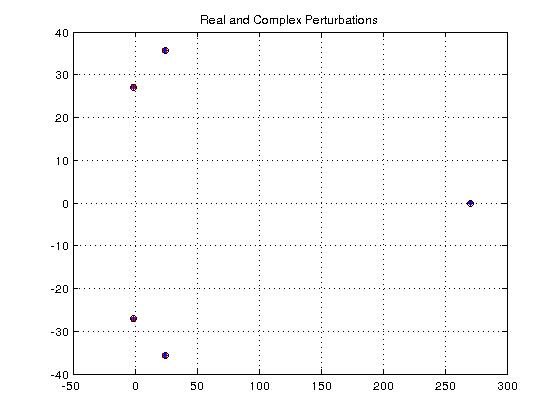
\includegraphics[width=0.5\textwidth]{1.jpg}
\caption{From the non defective matrix example.}
\end{figure}
\begin{figure}
\centering
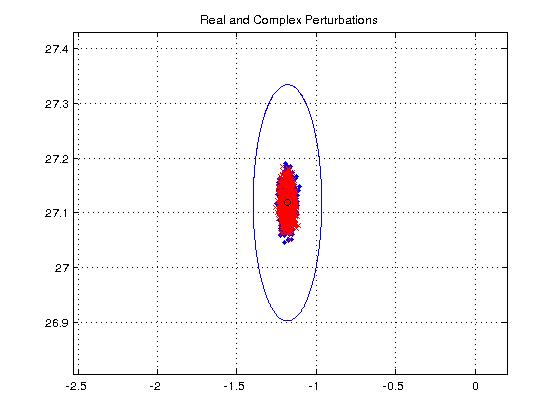
\includegraphics[width=0.5\textwidth]{2.jpg}
\caption{Close up from the non defective matrix example.}
\end{figure}
\begin{figure}
\centering
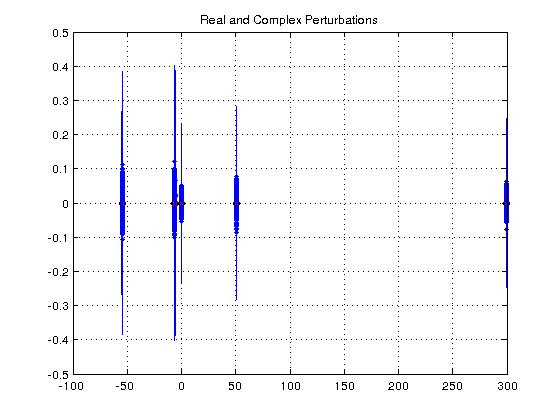
\includegraphics[width=0.5\textwidth]{degen2.jpg}
\caption{Defective matrix example.}
\end{figure}
\begin{figure}
\centering
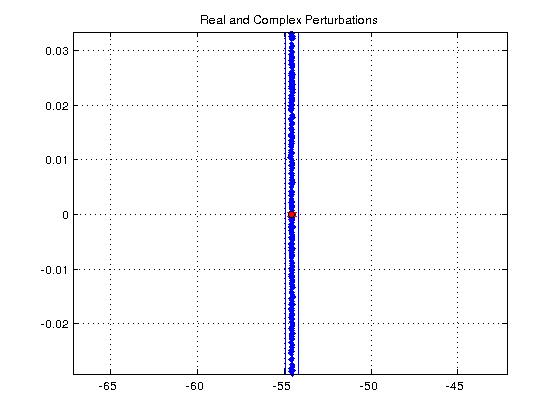
\includegraphics[width=0.5\textwidth]{degen2zoom.jpg}
\caption{Close up from the defective matrix example.}
\end{figure}
\end{center}

To answer the question \emph{What is the difference between the real perturbations and the complex perturbations?} I say that based on this example, there is no noticable difference between real and complex perturbations for a non-defective matrix. For a defective matrix, however, complex perturbations affect the computation of the eigenvalue much more than real perturbations. Compare the graphs of the perturbed eigenvalues for defective and non defective matrices in figures 1-4. Note: The circles drawn based upon theorem 4.4 only hold for simple eigenvalues. The close ups I show in this paper of circles around eigenvalues of defective matrices correspond to simple eigenvalues. I didnt have time to make sure that my code only plotted circles around the simple eigenvalues. Please trust that the close ups I show are of simple eigenvalues.

The following figures 5-8 will answer the question\emph{What happens to the regions occupied by the eigenvalues as the perturbation goes to zero?} We will see that the errors caused by complex perturbations are much worse than those caused by real perturbations for a defective matrix A, and that the errors caused by real and complex perturbations are very similar for both defective and non defective matrices. In either case, though, the area that the scattered eigenvalues cover shrinks as the error is tightened.

\begin{figure}
\centering
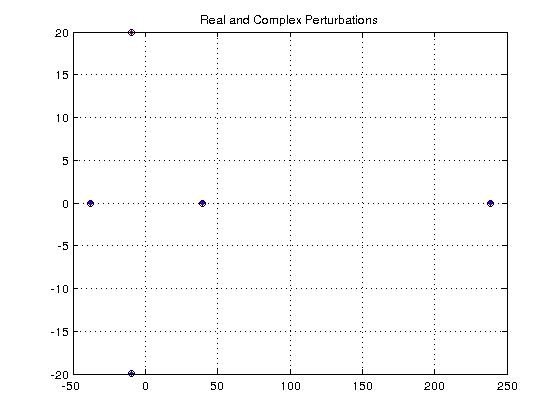
\includegraphics[width=0.5\textwidth]{1em8realout.jpg}
\caption{Nondefective matrix with err = 1e-8}
\end{figure}
\begin{figure}
\centering
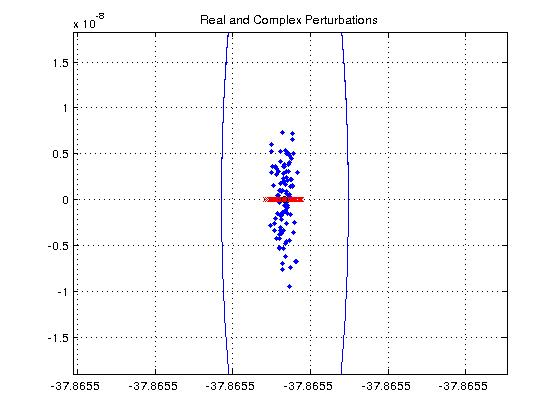
\includegraphics[width=0.5\textwidth]{1em8real.jpg}
\caption{Close up of figure 5}
\end{figure}
\begin{figure}
\centering
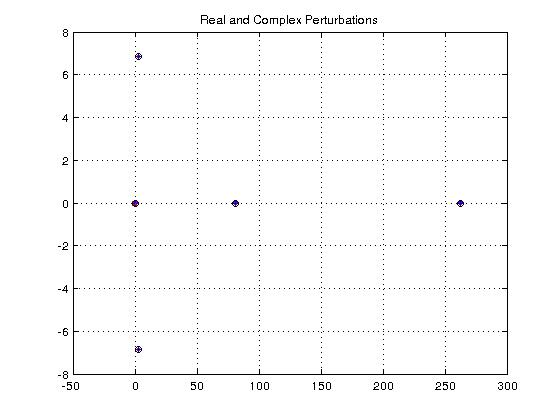
\includegraphics[width=0.5\textwidth]{1em8outdef.jpg}
\caption{Defective matrix shows more scattering by the complex perturbation (An order of magnitude greater than the nondefective case[see the close up])}
\end{figure}
\begin{figure}
\centering
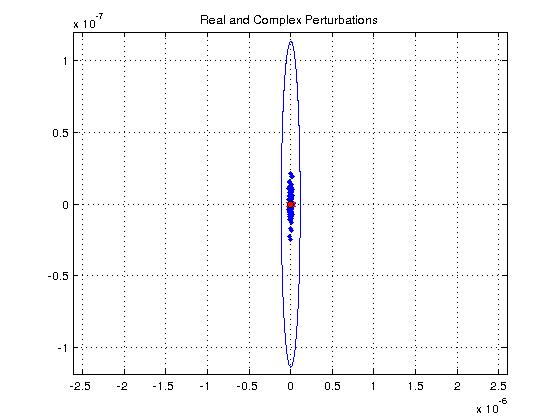
\includegraphics[width=0.5\textwidth]{1em8def.jpg}
\caption{Close up of figure 7}
\end{figure}
%%%%%%%%%%%%%%%%%%%%%%%%%%%%%%%%%%%%%%%%%%%%%%%%%%%%%%%%%%%%%%%%%%%%%%%%%%%%%%%%%%%%%%%%%%%%%%%%%%% QUESTION 4.15
%%%%%%%%%%%%%%%%%%%%%%%%%%%%%%%%%%%%%%%%%%%%%%%%%%%%%%%%%%%%%%%%%%%%%%%%%%%%%%%%%%%%%%%%%%%%%%%%%%
\item Problem 4.15\\
\emph{What happens if there are complex eigenvalues?}\\
If there are complex eigenvalues you get oscillations in the graph which do not go away. See figure 9. If all of the eigenvalues are real, then you get convergence. See figure 10.\\
\begin{figure}
\centering
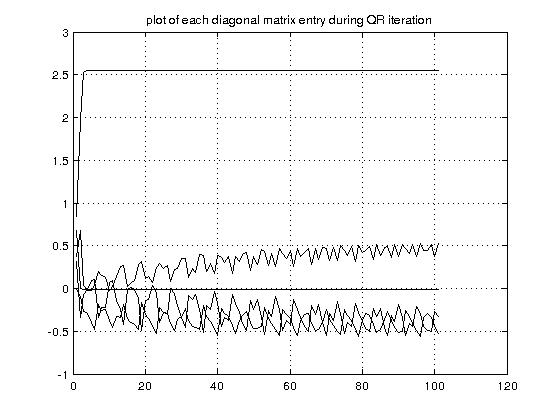
\includegraphics[width=0.5\textwidth]{oscillate.jpg}
\caption{Oscillation due to complex eigenvalues.}
\end{figure}
\begin{figure}
\centering
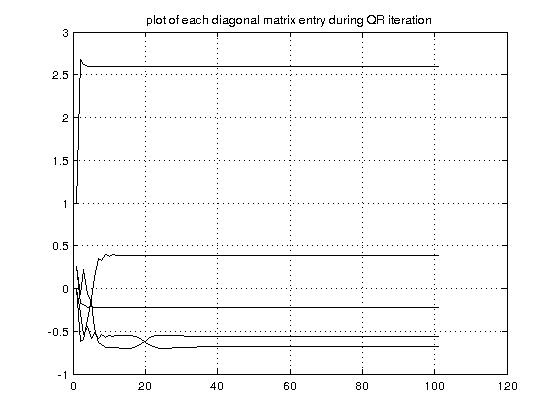
\includegraphics[width=0.5\textwidth]{nooscillate.jpg}
\caption{No oscillation since all eigenvalues are real.}
\end{figure}
\emph{In what order do the eigenvalues appear after many iterations?}\\
The eigenvalues appear in order of decreasing magnitude. See \textbf{Test Run} below for the function I used and the output of the function.
\begin{center}
\textbf{qrplt.m}
\begin{lstlisting}
function [a, r] = qrplt(a, m)
    hold off
    e=diag(a);
    for i=1:m,
       [q,r]=qr(a);dd=diag(sign(diag(r)));r=dd*r;q=q*dd;a=r*q; ...
       e=[e,diag(a)];
    end
    clf
    plot(e','k'),grid
    title('plot of each diagonal matrix entry during QR iteration')
    shg
end
\end{lstlisting}
\textbf{run\_qrplt.m}
\begin{lstlisting}
dim = 5;
A = rand(dim);
m = 100; % number of iterations.
[A,r] = qrplt(A, m);
disp('r:')
disp(r)
\end{lstlisting}
\textbf{Test Run}
\begin{lstlisting}
>> run_qr
r:
   2.5038e+00  -3.0672e-01  -1.6404e-01   2.4928e-01  -3.3548e-01
            0   7.6569e-01   1.4850e-01  -1.2838e-02   1.9286e-02
            0            0   4.0949e-01   7.2565e-01   3.6359e-01
            0            0            0   3.6432e-01   1.1508e-01
            0            0            0            0   2.4216e-01

>> eig(A)

ans =

   2.5038e+00
   7.6569e-01
  -4.0949e-01
  -3.6432e-01
   2.4216e-01           
\end{lstlisting}
\end{center}
\emph{How does this compare to the original value of a?}\\
After two sets of iterations and two flips, $A$ has not changed. This is in line with the analysis which you provided in the homework hints. \\
\begin{center}
\textbf{run\_qr.m}
\begin{lstlisting}
dim = 5;
perm=(dim:-1:1);
A = rand(dim); A = A'*A;
m = 5; % number of iterations.
lf = 2;
disp('original A:')
disp(A);
for flip = 1:lf
    A=qrplt(A, m);
    A=A(perm, perm);
    disp('Iterated and Flipped A:')
    disp(A);
    
end


\end{lstlisting}
\textbf{Results}
\begin{lstlisting}
>> run_qr
original A:
       1.4964       1.8069      0.71852       1.1274      0.46723
       1.8069       2.7447       1.2002       1.8077      0.82296
      0.71852       1.2002        1.016      0.73875      0.33798
       1.1274       1.8077      0.73875       1.6569      0.65332
      0.46723      0.82296      0.33798      0.65332      0.29895

Iterated and Flipped A:
     0.010221  -8.7224e-08  -3.8802e-10    7.471e-10   1.5814e-14
  -8.7224e-08      0.13825  -0.00074872    0.0010807   4.7329e-08
  -3.8802e-10  -0.00074872       0.5428    0.0025236  -2.5115e-06
    7.471e-10    0.0010807    0.0025236      0.47295   2.5708e-05
   1.5784e-14   4.7329e-08  -2.5115e-06   2.5708e-05       6.0487

Iterated and Flipped A:
       1.4963        1.807      0.71849       1.1276      0.46636
        1.807       2.7451       1.2003       1.8081      0.82177
      0.71849       1.2003        1.016       0.7389       0.3374
       1.1276       1.8081       0.7389       1.6574      0.65254
      0.46636      0.82177       0.3374      0.65254      0.29819
\end{lstlisting}
\end{center}
\emph{What do you get asymptotically?}\\
The diagonal elements go to the eigenvalues of A. The error goes to zero. Therefore the logarithm goes to negative infinity. There is no asymptotic behavior. Below are my code and a graph.
\begin{center}
\textbf{qrplt.m}
\begin{lstlisting}
function [a, err] = qrplt(a, m)
    hold off
    e=diag(a);
    for i=1:m,
       [q,r]=qr(a);dd=diag(sign(diag(r)));r=dd*r;q=q*dd;a=r*q; ...
       e=[e,diag(a)];
    end
    clf
    plot(e','k'),grid
    title('plot of each diagonal matrix entry during QR iteration')
    shg
    [~,c] = size(e);
    err = zeros((c-2), 1); 
    length(err)
    for col = 2:(c-1)
        err(col-1) = norm(e(:,m) - e(:,col))/norm(e(:,m));
    end
    length(err)
end	 	
\end{lstlisting}
\textbf{run\_qrplt.m}
\begin{lstlisting}
dim = 30;
A = rand(dim); A = A'*A;
m=1000;
[A,err] = qrplt(A,m);
plot(1:(m-1), log(err))
\end{lstlisting}
\begin{figure}
\centering
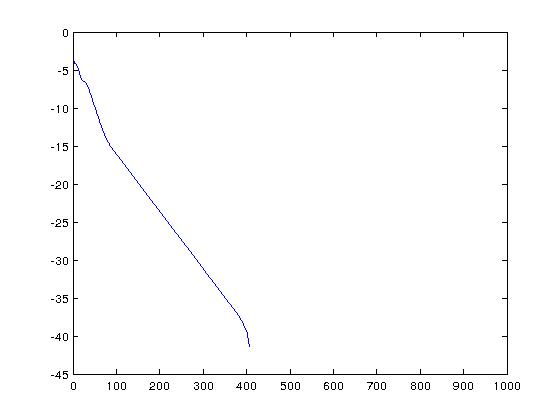
\includegraphics[width=0.5\textwidth]{noasymptote.jpg}
\caption{No Asymptote}
\end{figure}
\end{center}
\item Algorithm 5.2\\
\begin{center}
\textbf{dc\_eig.py}
\begin{lstlisting}
from numpy import array, zeros, ones, outer,  linspace, diag, dot, copy
from numpy import concatenate, finfo, multiply
from scipy.optimize import fsolve
from numpy.linalg import norm, eig
from scipy.linalg import block_diag 

def MakeTridiagonalMatrix(main, offset_one):
	"""This function will make a tridiagonal 2D array (NOT a matrix)
	which has the main array on its main diagonal and the offset_one 
	array on its super and sub diagonals.
	"""
	return diag(main) + diag(offset_one, k = -1) + diag(offset_one, k = 1)
	
def dc_eig(T):
	""" This function is a Python implementation of Dr. G. Hiary's 
	divide and conquer algorithm.
	"""
	eps = finfo(float).eps
	(n,m) = T.shape
	print n, m
	print n
	if(n==1):
		Q = array([1])
		L = T
		return Q, L
	else:
		m = n/2
		v = zeros(n)
		v[m-1:m+1] = 1
		rho = T[m-1][m]
		R = rho*outer(v,v)
		TT = T - R
		T1 = TT[0:m, 0:m]
		T2 = TT[m:, m:]
		(Q1, L1) = dc_eig(T1)
		(Q2, L2) = dc_eig(T2)
		
		D = block_diag(L1, L2)
		QQ = block_diag(Q1.T, Q2.T)
		u=dot(QQ,v)

		f = lambda x: 1 + rho*dot((multiply(u, 1/(diag(D)-x))),u)
		Ds = copy(diag(D)) # make a deep copy of the diag
		# sort now, otherwise the diagonal would be sorted in place
		Ds.sort()
		# reverse the list
		Ds[:] = Ds[::-1] 
		L = zeros((n,n))
		
		if(rho > 0):
			for i in range(0,n-1): 
				# Because Python is crazy, this will only go up to n-2.
				I = array([Ds[i+1]+eps, Ds[i] - eps])
				L[i+1][i+1] = fsolve(f, I)
			x0 = Ds[1] + eps
			if( f(x0) > 0):
				print 'Error 1 : cannot resolve zero of f'
				return
			x1 = x0
			while (f(x1) < 0):
				x1 = x1 + 0.1			
			L[0][0] = fsolve(f, array([x0, x1]))
		else:
			for i in range(0,n-1):
				I = array([Ds[i+1]+eps, Ds[i] - eps])
				L[i][i] = fsolve(f, I)
			x0 = Ds[n] - eps
			if(f(x0) > 0):
				print('Error 2: cannot resolve zero of f')
				return
			x1 = x0
			while (f(x1) < 0):
				x1 = x1 - 0.1
			L[n][n] = fsolve(f, array([x1, x0]))
		Qprime = full((n, n), nan)
		for i in range (0, n):
			alpha = L[i][i]
			qi = u/(diag(D) - alpha) 
			# I think python defaults to itemwise division
			qi = qi/norm(qi)
			Qprime[:,i] = qi
			Q = block_diag(Q1, Q2)*Qprime
		return Q,L

main = linspace(-10,10, 5)
off = linspace(-1,6,4)
T = MakeTridiagonalMatrix(main, off)
(Q,L) = dc_eig(T)
\end{lstlisting}
\end{center}
Unfortunately, I am unable to finish this because Python does not have the equivalent of the MATLAB fzero() function. This semester I have found that Python has no fzero() and that there is no routine for animated 3d plotting, as MATLAB has. These are both problems that are waiting to be solved by a motivated person.
\end{enumerate}

\end{document}